% handout
\documentclass[11pt,final,usepdftitle=false]{beamer}
\mode<presentation>
\usetheme{ln12en}
\graphicspath{{\logopath}{\picspath}{\figspath}{./logos/}{./pics/}{./figs/}}
\usepackage{listings}
%\usepackage{bera}
\usepackage{inconsolata}
\usepackage{moresize}
\usepackage{ucs}
\usepackage{framed}
\usepackage{adjustbox}
%\renewcommand*\ttdefault{cmvtt}


\hypersetup{pdftitle={Lucas Nussbaum - systemd}}
\title{systemd}
\authorteaching
\instituteiutlp
\newcommand{\tilda}{\textasciitilde{}}
\date{}


% \AtBeginSection[]
% {
%   \begin{frame}
%     \frametitle{Outline}
%     \tableofcontents[currentsection]
%   \end{frame}
% }

\usepackage{tikz}
\usetikzlibrary{shapes,arrows,positioning}
\newcommand{\Gentsroom}{{\fontfamily{mvs}\fontencoding{U}\fontseries{m}\fontshape{n}\selectfont\char120}}

\begin{document}

\frame{\titlepage}

\begin{frame}{Outline}
	\tableofcontents
\end{frame}

\section{Introduction}

\begin{frame}{Init system}
\begin{itemize}
\item First process started by the kernel (pid 1)
	\hbr
\item Responsible for \alert{bringing up the rest of userspace}
	\begin{itemize}
		\item Mounting filesystems
		\item Starting services
		\item \ldots
	\end{itemize}
	\hbr
\item Also the parent for orphan processes
	\hbr
\item Traditional init system on Linux: \alert{sysVinit}
	\begin{itemize}
		\item Inherited from Unix System V
		\item With additional tools (insserv, startpar) to handle dependencies and parallel initialization
	\end{itemize}
\end{itemize}
\end{frame}

\begin{frame}{systemd}
	\begin{itemize}
		\item Written (since 2010) by Lennart Poettering (Red Hat) and others
			\hbr
		\item Now the default on most Linux distributions
			\hbr
		\item Shifts the scope from \textsl{starting all services} (sysVinit) to\\
			\alert{managing the system and all services}
			\hbr
		\item Key features:
			\begin{itemize}
				\item Relies on cgroups for
					\begin{itemize}
						\item Services supervision
						\item Control of services execution environment
					\end{itemize}
					\hbr
				\item Declarative syntax for unit files $\leadsto$ more efficient/robust
					\hbr
				\item Socket activation for parallel services startup
					\hbr
				\item Nicer user interface (systemctl \& friends)
			\end{itemize}
			\hbr
		\item Additional features: logging, timer units (cron-like), user sessions handling, containers management
	\end{itemize}
\end{frame}

\section{Behind the scenes: cgroups}

\begin{frame}{Behind the scenes: cgroups}
\begin{itemize}
\item Abbreviated from \textsl{control groups}
\hbr
\item Linux kernel feature
\hbr
\item Limit, account for and isolate \alert{processes and their resource usage} (CPU, memory, disk I/O, network, etc.)
\hbr
\item Related to \alert{namespace isolation}:
	\begin{itemize}
		\item Isolate processes from the rest of the system
			\hbr
		\item \textsl{Chroots on steroids}
			\hbr
		\item PID, network, UTS, mount, user, etc.
	\end{itemize}
			\hbr
		\item LXC, Docker $\approx$ cgroups + namespaces (+ management tools)
\end{itemize}
\end{frame}

\begin{frame}{cgroups and systemd}
	\begin{itemize}
		\item \alert{Each service runs in its own cgroup}
		\hhbr
	\item Enables:
		\begin{itemize}
			\item Tracking and killing all processes created by each service
				\hhbr
			\item Per-service accounting and resources allocation/limitation
		\end{itemize}
		\hhbr
	\item Previously, with sysVinit:
		\begin{itemize}
			\item No tracking of which service started which processes
				\begin{itemize}
					\item PID files, or hacks in init scripts: \texttt{pidof} / \texttt{killall} / \texttt{pgrep}
						\hhbr
					\item Hard to completely terminate a service (left-over CGI scripts when killing Apache)
				\end{itemize}
				\hbr
			\item No resources limitation (or using \texttt{setrlimit} (= \texttt{ulimit}), which is per-process, not per-service)
		\end{itemize}
	\hhbr
	\item \alert{Also isolate user sessions} $\leadsto$ kill all user processes (not by default)
	\hhbr
\item More information: \href{http://0pointer.net/blog/projects/cgroups-vs-cgroups.html}{\ul{Control Groups vs. Control Groups}} and\\ \href{http://0pointer.net/blog/projects/systemd-for-admins-2.html}{\ul{Which Service Owns Which Processes?}}
\end{itemize}
\end{frame}



\begin{frame}{\texttt{systemd-cgls}: visualizing the cgroups hierarchy}
% export GTK_MODULES=/usr/lib/gtk-3.0/modules/libgtk-vector-screenshot.so
% take-vector-screenshot
\hbr

\includegraphics[height=0.9\textheight]{figs/systemd-cgls}
\end{frame}

\begin{frame}{\texttt{systemd-cgtop}: per-service resources usage}
\begin{framed}

\includegraphics[width=1\textwidth]{figs/systemd-cgtop}
\end{framed}
Requires enabling \texttt{CPUAccounting}, \texttt{BlockIOAccounting}, \texttt{MemoryAccounting}
\end{frame}

\section{Managing services}

\begin{frame}{Managing services with \texttt{systemctl}}
	\begin{itemize}
		\item What is being manipulated is called a  \alert{\textsl{unit}}: services (.service), mount points (.mount), devices (.device), sockets (.socket), etc.
			\hbr
		\item Basic commands:
\hbr
	\end{itemize}
	\resizebox{\textwidth}{!}{
	\begin{tabular}{|c|c|c|}
		\hline
		sysVinit & systemd & notes \\
		\hline
		service foo start & systemctl start foo & \\
		service foo stop & systemctl stop foo & \\
		service foo restart & systemctl restart foo & \\
		service foo reload & systemctl reload foo & \\
		service foo condrestart & systemctl condrestart foo & restart if already running \\
		update-rc.d foo enable & systemctl enable foo & auto-start at next boot \\
		update-rc.d foo disable & systemctl disable foo & disable auto-start \\
		& systemctl is-enabled foo & \\
		\hline
	\end{tabular}}
	\begin{itemize}
		\item There's auto-completion (\texttt{apache2} and \texttt{apache2.service} work)
		\hbr
		\item Several services can be specified:\\
			\texttt{systemctl restart apache2 postgresql}
		\hbr
	\end{itemize}
\end{frame}

\begin{frame}{systemd and runlevels}
	\begin{itemize}
		\item With sysVinit, runlevels control which services are started automatically
			\begin{itemize}
				\item 0 = halt; 1 = single-user / minimal mode; 6 = reboot
				\item Debian: no difference by default between levels 2, 3, 4, 5
				\item RHEL: 3 = multi-user text, 5 = multi-user graphical
			\end{itemize}
			\hbr
		\item systemd replaces runlevels with \alert{targets}:
			\begin{itemize}
				\item Configured using symlinks farms in \texttt{/etc/systemd/system/\textbf{target}.wants/}
					\hbr
				\item \texttt{systemctl enable}/\texttt{disable} manipule those symlinks
					\hbr
				\item \texttt{systemctl mask} disables the service and prevents it from being started manually
					\hbr
				\item The default target can be configured with\\ \texttt{systemctl get-default/set-default}
					\hbr
				\item More information: \href{http://0pointer.net/blog/projects/three-levels-of-off.html}{\ul{The Three Levels of "Off"}}
			\end{itemize}
	\end{itemize}
\end{frame}

\begin{frame}[fragile]{Default targets (\texttt{bootup(7)})}
\begin{center}
\begin{adjustbox}{height=0.45\textheight,keepaspectratio}
\begin{lstlisting}[basicstyle=\ttfamily\tiny,escapeinside={<<}]
local-fs-pre.target
         |
         v
(various mounts and   (various swap   (various cryptsetup
 fsck services...)     devices...)        devices...)       (various low-level   (various low-level
         |                  |                  |             services: udevd,     API VFS mounts:
         v                  v                  v             tmpfiles, random     mqueue, configfs,
  local-fs.target      swap.target     cryptsetup.target    seed, sysctl, ...)      debugfs, ...)
         |                  |                  |                    |                    |
         \__________________|_________________ | ___________________|____________________/
                                              \|/
                                               v
                                        sysinit.target
                                               |
          ____________________________________/|\________________________________________
         /                  |                  |                    |                    \
         |                  |                  |                    |                    |
         v                  v                  |                    v                    v
     (various           (various               |                (various          rescue.service
    timers...)          paths...)              |               sockets...)               |
         |                  |                  |                    |                    v
         v                  v                  |                    v               <\textbf{rescue.target}<
   timers.target      paths.target             |             sockets.target
         |                  |                  |                    |
         \__________________|_________________ | ___________________/
                                              \|/
                                               v
                                         basic.target
                                               |
          ____________________________________/|                                 emergency.service
         /                  |                  |                                         |
         |                  |                  |                                         v
         v                  v                  v                                  <\textbf{emergency.target}<
     display-        (various system    (various system
 manager.service         services           services)
         |             required for            |
         |            graphical UIs)           v
         |                  |            <\textbf{multi-user.target}<
         |                  |                  |
         \_________________ | _________________/
                           \|/
                            v
                      <\textbf{graphical.target}<
\end{lstlisting}
\end{adjustbox}
\end{center}
\end{frame}

\section{Analyzing startup performance}

\begin{frame}[fragile]{Analyzing startup performance}
	\begin{itemize}
		\item Fast boot matters in some use-cases:

			\begin{itemize}
				\item Virtualization, Cloud:
					\begin{itemize}
						\item Almost no BIOS / hardware checks $\leadsto$ only software startup
							\hbr
						\item Requirement for infrastructure elasticity
					\end{itemize}
					\hbr
				\item Embedded world
			\end{itemize}
			\hbr
		\item \texttt{systemd-analyze time}: summary
	\end{itemize}
	\begin{lstlisting}[basicstyle=\ttfamily\scriptsize,escapeinside={||}]
	Startup finished in 4.883s (kernel) + 5.229s (userspace) = 10.112s
	\end{lstlisting}
	\begin{itemize}
			\hbr
		\item \texttt{systemd-analyze blame}: worst offenders
			\begin{lstlisting}[basicstyle=\ttfamily\normalsize,escapeinside={||}]
			2.417s systemd-udev-settle.service
			2.386s postgresql@9.4-main.service
			1.507s apache2.service
			240ms NetworkManager.service
			236ms ModemManager.service
			194ms accounts-daemon.service
			\end{lstlisting}
	\end{itemize}
\end{frame}

\begin{frame}{systemd-analyze plot}
	\hbr
	\begin{itemize}
		\item Similar to bootchartd, but does not require rebooting with a custom \texttt{init=} kernel command-line
	\end{itemize}
	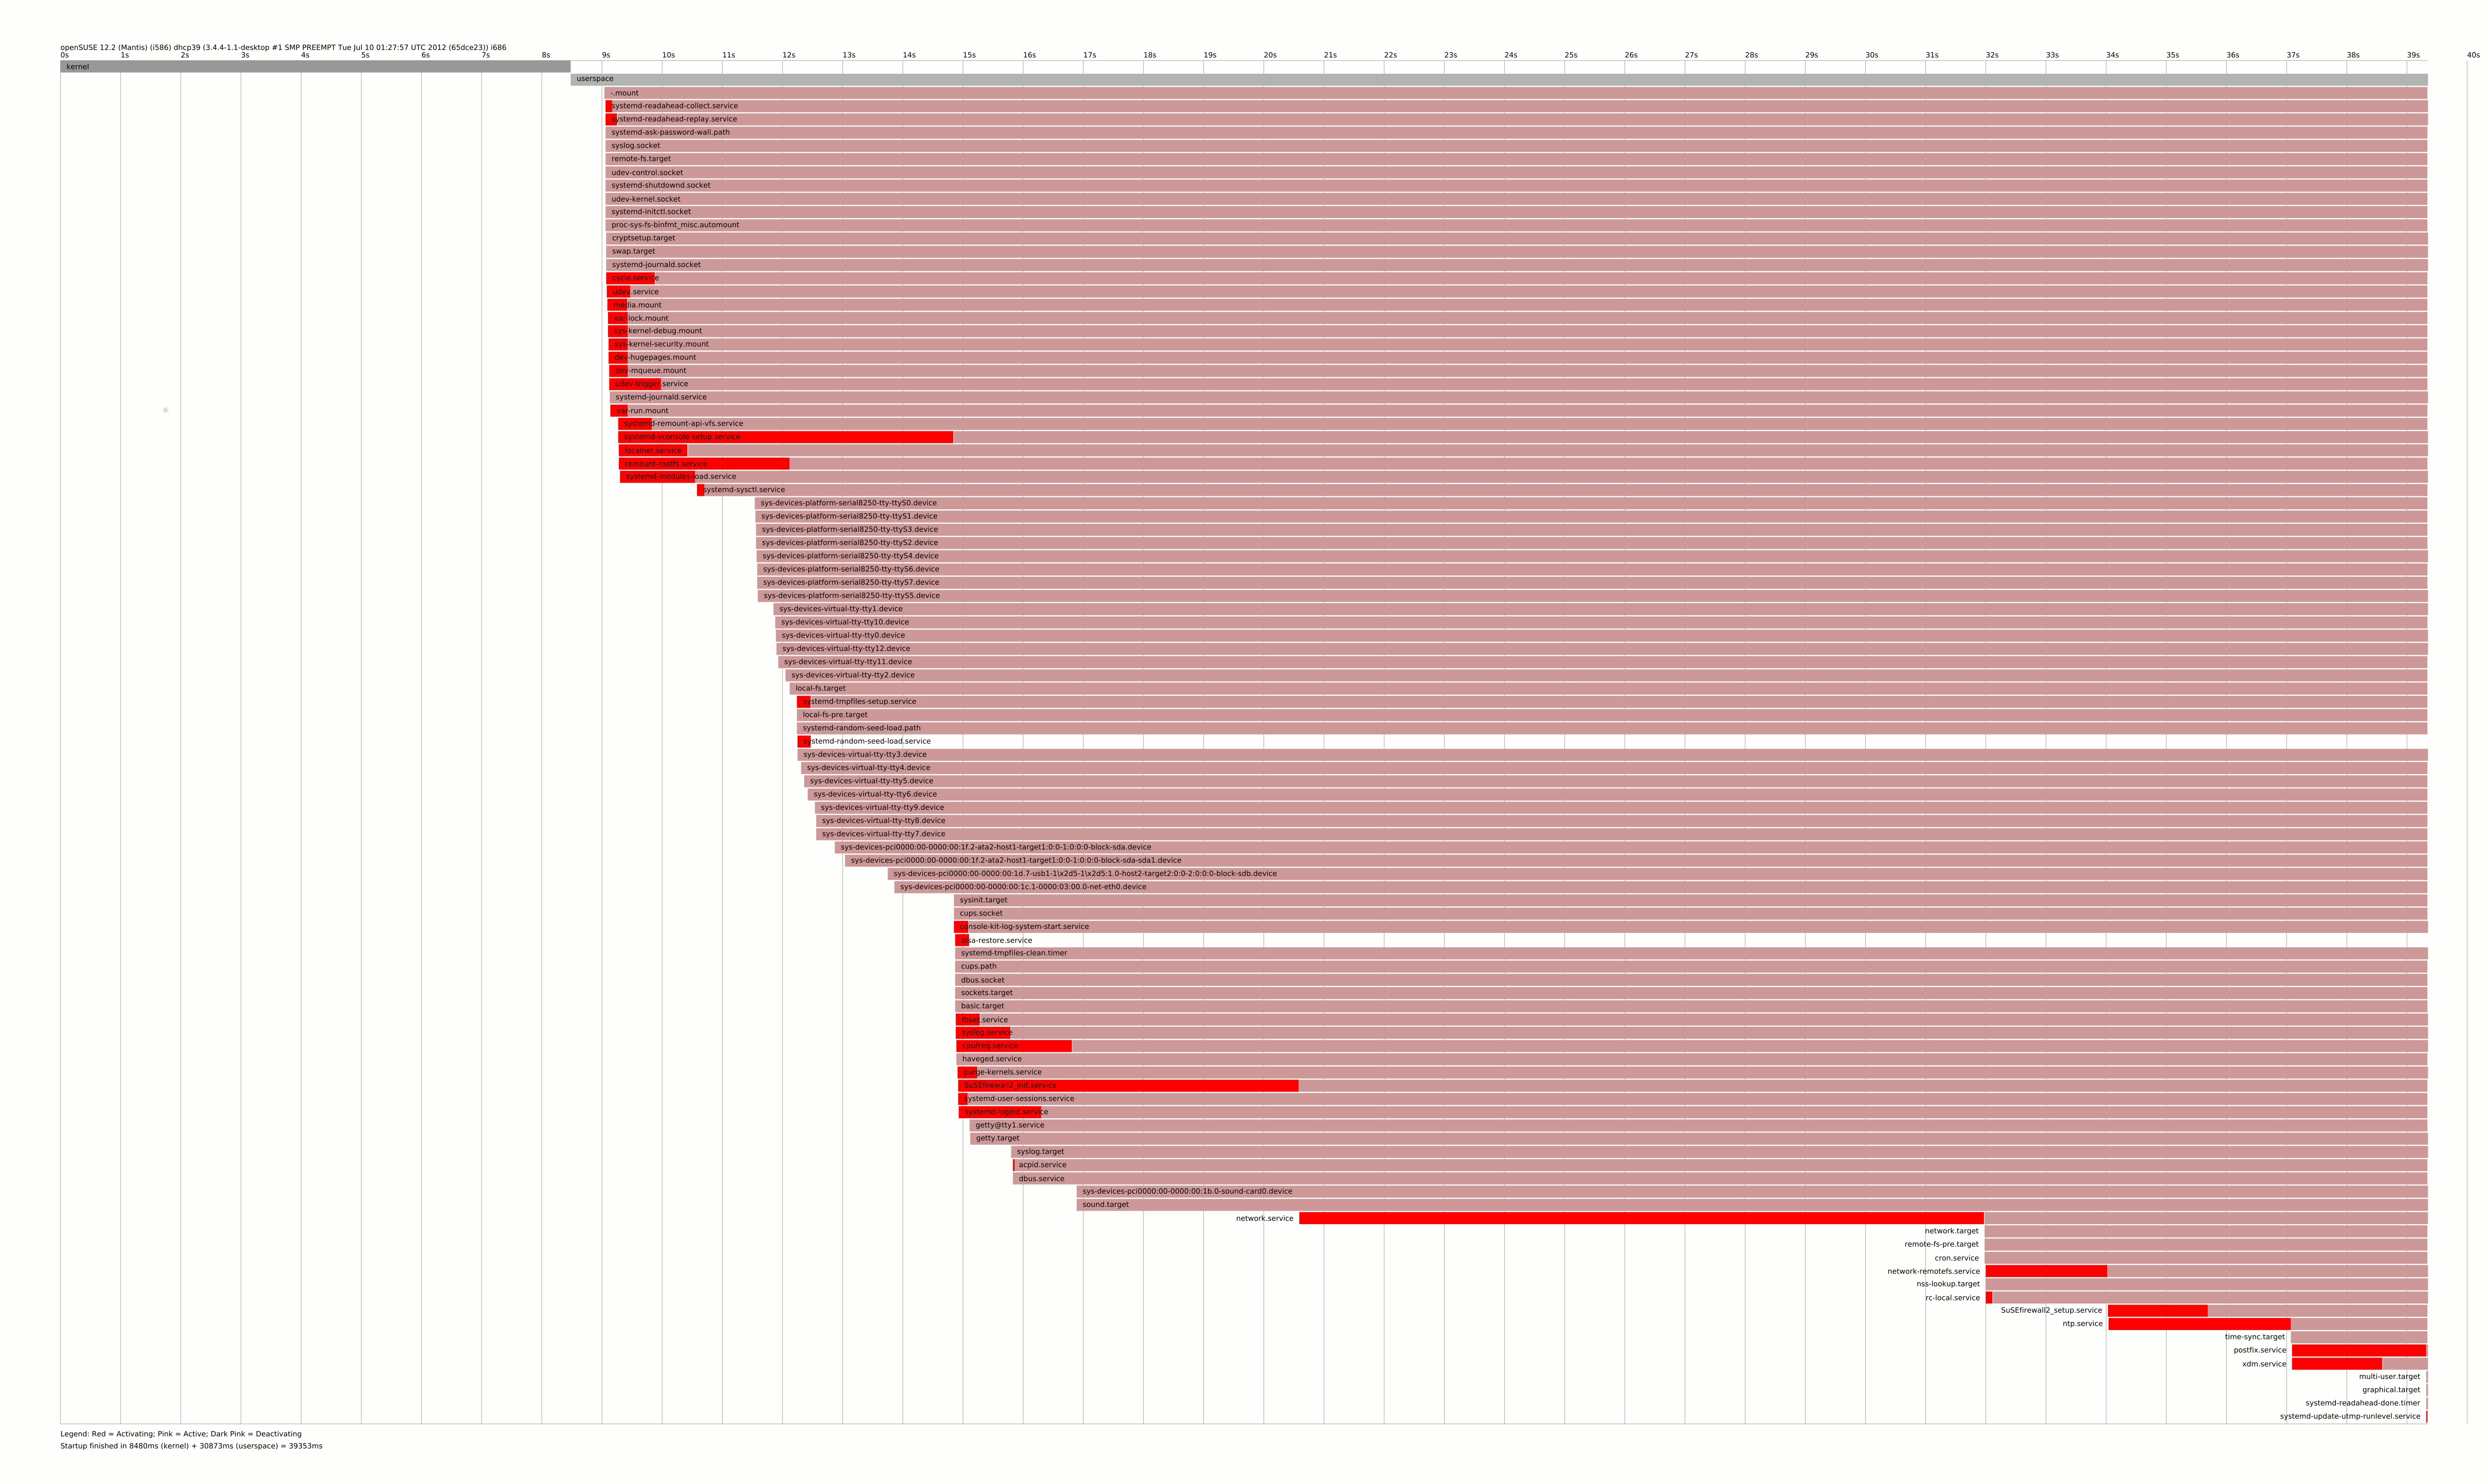
\includegraphics[width=\textwidth]{figs/systemd-analyze-plot.png}
\end{frame}

\begin{frame}[fragile]{systemd-analyze critical-chain}
	\begin{itemize}
		\item Shows services in the critical path
	\end{itemize}
	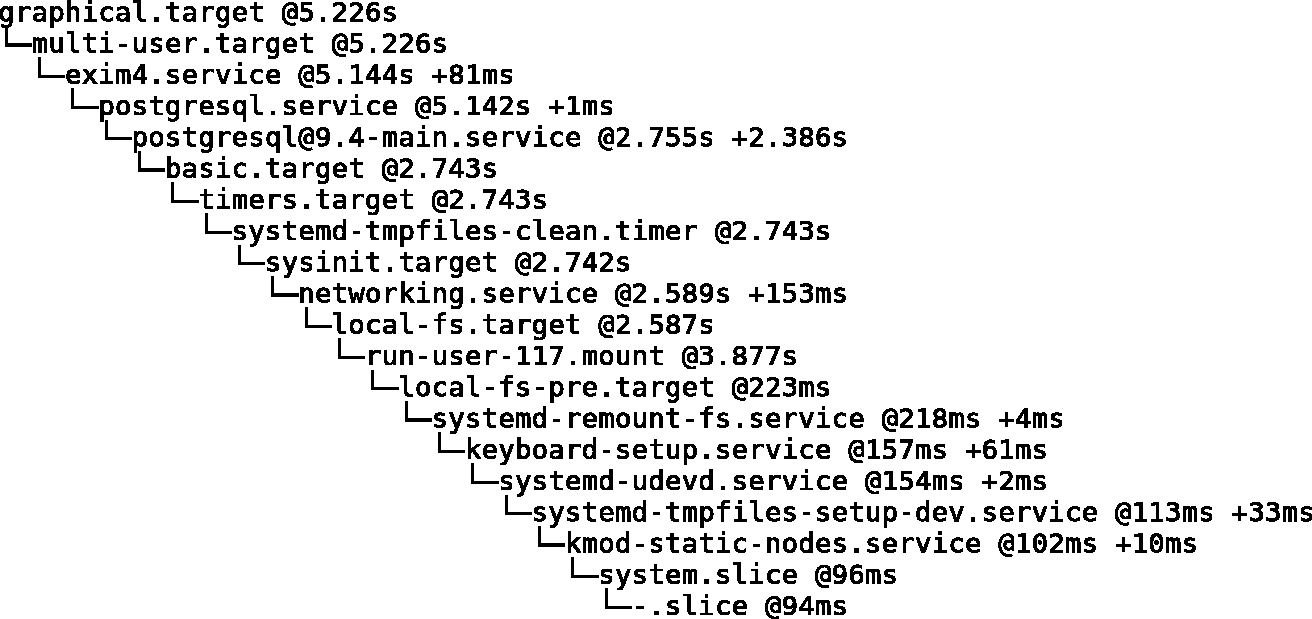
\includegraphics[width=\textwidth]{figs/systemd-analyze-critical-chain.pdf}
\end{frame}

\section{Exploring the system status}

\begin{frame}{Exploring the system status}
\begin{itemize}
\item Listing units with \texttt{systemctl list-units} (or just \texttt{systemctl}):
\begin{itemize}
\item active units: \texttt{systemctl}
\hhbr
\item List only services: \texttt{systemctl -t service}
\hhbr
\item List units in failed state: \texttt{systemctl --failed}
\end{itemize}
\hbr
\item Whole system overview: \texttt{systemctl status}
\hbr
\item GUI available: \texttt{systemadm}
\end{itemize}
\end{frame}

\begin{frame}{\texttt{systemctl status \textsl{\tt service}}}
\br
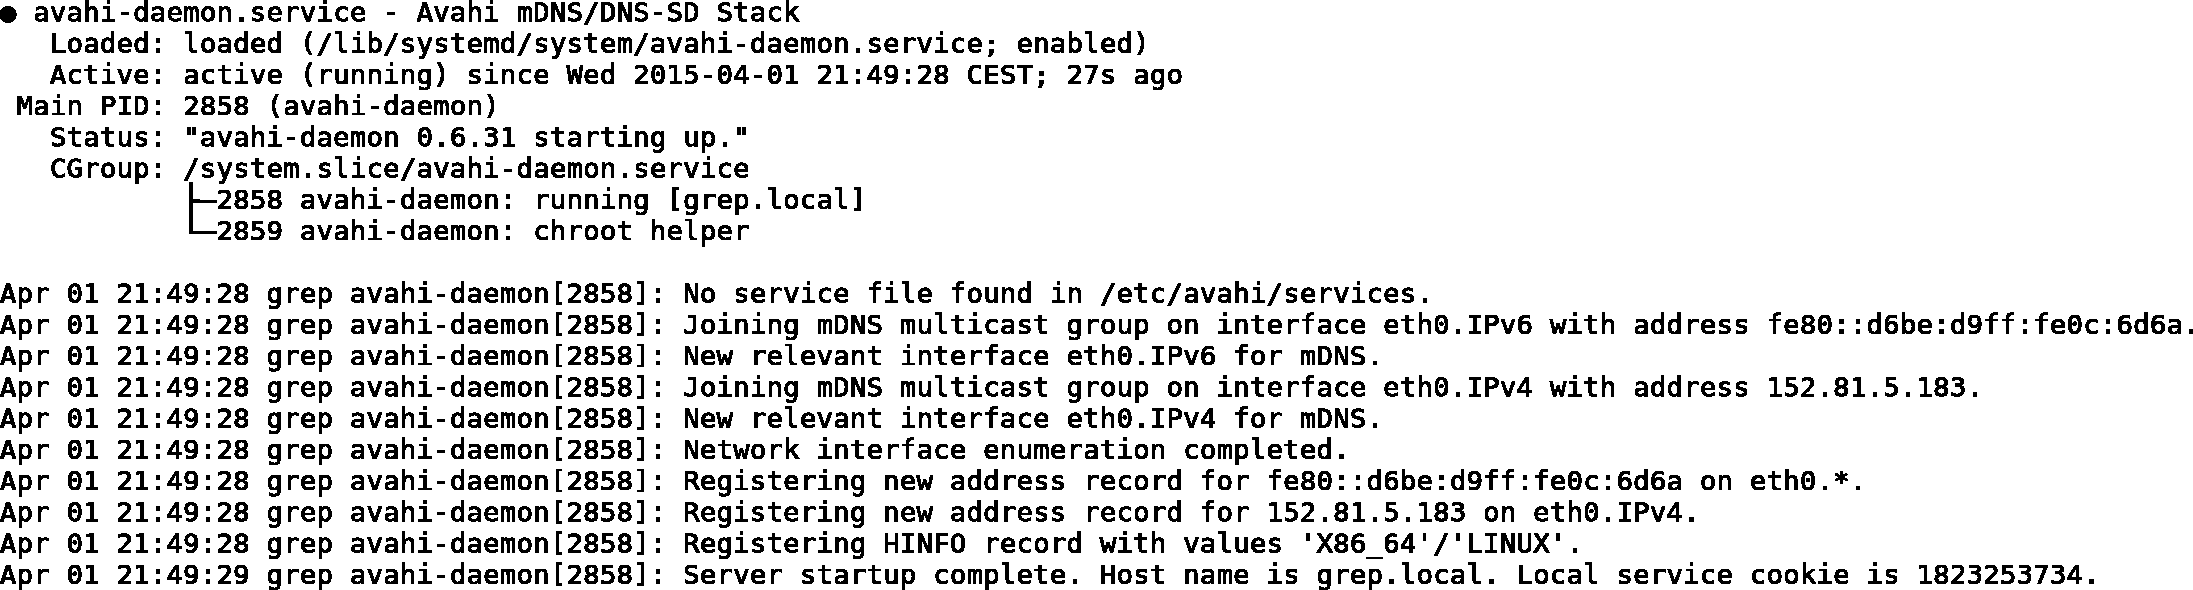
\includegraphics[width=1.5\textwidth]{figs/systemctl-status}
\hbr
Includes:
\begin{itemize}
\item Service name and description, state, PID
\item Free-form status line from \texttt{systemd-notify(1)} or \texttt{sd\_notify(3)}
\item Processes tree inside the cgroup
\item Last lines from journald (syslog messages and stdout/stderr)
\end{itemize}
\end{frame}

\section{Configuring services by writing unit files}

\begin{frame}{Configuring services by writing unit files}
\begin{itemize}
\item With sysVinit: shell scripts in \texttt{/etc/init.d/}
\begin{itemize}
\item Long and difficult to write
	\hbr
\item Redundant code between services
	\hbr
\item Slow (numerous \texttt{fork()} calls)
\end{itemize}
\hbr
\item \alert{With systemd: declarative syntax} (.desktop-like)
\begin{itemize}
\item Move intelligence from scripts to systemd
	\hbr
\item Covers most of the needs, but shell scripts can still be used
	\hbr
\item Can use includes and overrides (\texttt{systemd-delta})
	\hbr
\item View config file for a unit: \texttt{systemctl cat atd.service}
	\hbr
\item Or just find the file under \texttt{/lib/systemd/system/} (distribution's defaults) or \texttt{/etc/systemd/system} (local overrides)
\end{itemize}
\end{itemize}
\end{frame}

\begin{frame}[fragile]{Simple example: atd}
\begin{lstlisting}[basicstyle=\ttfamily\normalsize,escapeinside={||}]
[Unit]
Description=Deferred execution scheduler
|\alert{\# Pointer to documentation shown in systemctl status}|
Documentation=man:atd(8)

[Service]
|\alert{\# Command to start the service}|
ExecStart=/usr/sbin/atd -f
IgnoreSIGPIPE=false |\alert{\# Default is true}|

[Install]
|\alert{\# Where "systemctl enable" creates the symlink}|
WantedBy=multi-user.target
\end{lstlisting}
\end{frame}

\begin{frame}[fragile]{Common options}
\hbr
\begin{itemize}
	\item \alert{Documented in \texttt{systemd.unit(5)}} ([Unit]), \alert{\texttt{systemd.service(5)}} ([Service]), \alert{\texttt{systemd.exec(5)}} (execution environment)
\hbr
\item \alert{Show all options} for a given service:\\
	\alert{\texttt{systemctl show atd}}
\hbr
	\item Sourcing a configuration file:\\
\texttt{EnvironmentFile=-/etc/default/ssh}\\
\texttt{ExecStart=/usr/sbin/sshd -D \$SSHD\_OPTS}
\hbr
\item Using the \texttt{\$MAINPID} magic variable:\\
\texttt{ExecReload=/bin/kill -HUP \$MAINPID}
\hbr
\item Auto-restart a service when crashed: ($\approx$ runit / monit)\\
\texttt{Restart=on-failure}
\hbr
\item Conditional start:\\
\texttt{ConditionPathExists=!/etc/ssh/sshd\_not\_to\_be\_run}\\
{\small Conditions on architecture, virtualization, kernel~cmdline, AC~power, etc.}
\end{itemize}
\end{frame}

\begin{frame}{Options for isolation and security}
	\begin{itemize}
		\item Use a \alert{network namespace} to isolate the service from the network:\\
			\texttt{PrivateNetwork=yes}
			\hbr
		\item Use a \alert{filesystem namespaces}:
			\begin{itemize}
				\item To provide a service-specific \texttt{/tmp} directory:\\
					\texttt{PrivateTmp=yes}
					\hbr
				\item To make some directories inaccessible or read-only:\\
					\texttt{InaccessibleDirectories=/home}\\
					\texttt{ReadOnlyDirectories=/var}
			\end{itemize}
			\hbr
		\item Specify the list of \alert{\texttt{capabilities(7)}} for a service:\\
			\texttt{CapabilityBoundingSet=CAP\_CHOWN CAP\_KILL}\\
			Or just remove one:\\
			\texttt{CapabilityBoundingSet=\textasciitilde{}CAP\_SYS\_PTRACE}
			\hbr
		\item Disallow forking:\\
			\texttt{LimitNPROC=1}
	\end{itemize}
\end{frame}
\begin{frame}{Options for isolation and security (2)}
\begin{itemize}
		\item Run as user/group: \texttt{User=}, \texttt{Group=}
			\hbr
		\item Run service inside a chroot:\\
			\texttt{RootDirectory=/srv/chroot/foobar}\\
			\texttt{ExecStartPre=/usr/local/bin/setup-foobar-chroot.sh}\\
			\texttt{ExecStart=/usr/bin/foobard}\\
			\texttt{RootDirectoryStartOnly=yes}
			\hbr
		\item Control CPU shares, memory limits, block I/O, swapiness:\\
			\texttt{CPUShares=1500}\\
			\texttt{MemoryLimit=1G}\\
			\texttt{BlockIOWeight=500}\\
			\texttt{BlockIOReadBandwith=/var/log 5M}\\
			\texttt{ControlGroupAttribute=memory.swappiness 70}
			\hbr
		\item More information:
				\href{http://0pointer.net/blog/projects/systemd-for-admins-3.html}{\ul{Converting sysV init scripts to systemd service files}},
				\href{http://0pointer.net/blog/projects/security.html}{\ul{Securing your services}},
				\href{http://0pointer.net/blog/projects/changing-roots.html}{\ul{Changing roots}},
				\href{http://0pointer.net/blog/projects/resources.html}{\ul{Managing resources}}
	\end{itemize}
\end{frame}

\section{Timer units}

\begin{frame}{Timer units}
	\begin{itemize}
		\item Similar to cron, but with all the power of systemd (dependencies, execution environment configuration, etc)
		\hbr
	\item \alert{Realtime (wallclock) timers}: calendar event expressions
			\begin{itemize}
				\item Expressed using a complex format (see \texttt{systemd.time(7)}), matching timestamps like:
					\texttt{Fri 2012-11-23 11:12:13}
				\hbr
			\item Examples of valid values:  \texttt{hourly} (= \texttt{*-*-* *:00:00}), \texttt{daily} (= \texttt{*-*-* 00:00:00}), \texttt{*:2/3} (= \texttt{*-*-* *:02/3:00})
		\end{itemize}
		\hbr
	\item \alert{Monotonic timers}, relative to different starting points:
		\begin{itemize}
			\item 5 hours and 30 mins after system boot: \texttt{OnBootSec=5h 30m}
				\hbr
			\item 50s after systemd startup: \texttt{OnstartupSec=50s}
				\hbr
			\item 1 hour after the unit was last activated: \texttt{OnUnitActiveSec=1h}\\
				(can be combined with \texttt{OnBootSec} or \texttt{OnStartupSec} to ensure that a unit runs on a regular basis)
		\end{itemize}
	\end{itemize}
\end{frame}

\begin{frame}[fragile]{Timer units example}
\begin{itemize}
\item \texttt{myscript.service}:
\begin{lstlisting}[basicstyle=\ttfamily\footnotesize,escapeinside={||}]
[Unit]
Description=MyScript

[Service]
Type=simple
ExecStart=/usr/local/bin/myscript
\end{lstlisting}
\item \texttt{myscript.timer}:
\begin{lstlisting}[basicstyle=\ttfamily\footnotesize,escapeinside={||}]
[Unit]
Description=Runs myscript every hour

[Timer]
# Time to wait after booting before we run first time
OnBootSec=10min
# Time between running each consecutive time
OnUnitActiveSec=1h
Unit=myscript.service

[Install]
WantedBy=multi-user.target
\end{lstlisting}
\end{itemize}
\end{frame}
\begin{frame}{Timer units example (2)}
	\begin{itemize}
\item Start timer:\\ \texttt{systemctl start myscript.timer}
	\hbr
\item Enable timer to start at boot:\\
	\texttt{systemctl enable myscript.timer}
\hbr
\item List all timers:\\ \texttt{systemctl list-timers}
\end{itemize}
\end{frame}

\section{Socket activation}

\begin{frame}{Socket activation}
\begin{itemize}
\item systemd listens for connection on behalf of service until the service is ready, then passes pending connections
\hbr
\item Benefits:
	\begin{itemize}
		\item \alert{No need to express ordering of services during boot}:
			\begin{itemize}
				\item They can all be started in parallel $\leadsto$ \alert{faster boot}
				\item And they will wait for each other when needed (when they will talk to each other), thanks to socket activation
			\end{itemize}
			\hbr
		\item Services that are \alert{seldomly used do not need to keep running}, and can be started on-demand
\end{itemize}
\hbr
\item Not limited to network services: also D-Bus activation and path activation
\hbr
\item More information: \href{http://0pointer.net/blog/projects/inetd.html}{\ul{Converting inetd Service}}, \href{http://0pointer.net/blog/projects/socket-activation.html}{\ul{Socket Activation for developers}} (+ \href{http://0pointer.net/blog/projects/socket-activation2.html}{\ul{follow-up}})
\end{itemize}
\end{frame}

\begin{frame}[fragile]{Socket activation example: dovecot}
\begin{columns}[t]
\begin{column}{0.41\textwidth}
	\alert{\texttt{dovecot.socket}:}
\begin{lstlisting}[basicstyle=\ttfamily\scriptsize,escapeinside={||}]
[Unit]
Description=Dovecot IMAP/POP3 \
 email server activation socket

[Socket]
# dovecot expects separate
# IPv4 and IPv6 sockets
BindIPv6Only=ipv6-only
ListenStream=0.0.0.0:143
ListenStream=[::]:143
ListenStream=0.0.0.0:993
ListenStream=[::]:993
KeepAlive=true

[Install]
WantedBy=sockets.target
\end{lstlisting}
\end{column}
\begin{column}{0.49\textwidth}
\alert{\texttt{dovecot.service}:}
\begin{lstlisting}[basicstyle=\ttfamily\scriptsize,escapeinside={||}]
[Unit]
Description=Dovecot IMAP/POP3 \
 email server
After=local-fs.target network.target

[Service]
Type=simple
ExecStart=/usr/sbin/dovecot -F
NonBlocking=yes

[Install]
WantedBy=multi-user.target
\end{lstlisting}
\end{column}
\end{columns}
\end{frame}

\begin{frame}[fragile]{Socket activation example: sshd}
\begin{itemize}
\item \texttt{sshd.socket}:
\begin{lstlisting}[basicstyle=\ttfamily\footnotesize,escapeinside={||}]
[Unit]
Description=SSH Socket for Per-Connection Servers

[Socket]
ListenStream=22
Accept=yes

[Install]
WantedBy=sockets.target
\end{lstlisting}
\item \texttt{sshd@.service}:
\begin{lstlisting}[basicstyle=\ttfamily\footnotesize,escapeinside={||}]
[Unit]
Description=SSH Per-Connection Server

[Service]
ExecStart=-/usr/sbin/sshd -i
StandardInput=socket
\end{lstlisting}
\end{itemize}
\end{frame}

\begin{frame}[fragile]{Socket activation example: sshd (2)}
\begin{itemize}
	\item \texttt{sshd@.service} means that this is an \alert{instantiated service}
	\hbr
\item There's one instance of \texttt{sshd@.service} per connection:
\end{itemize}
\begin{lstlisting}[basicstyle=\ttfamily\scriptsize]
# systemctl --full | grep ssh
sshd@172.31.0.52:22-172.31.0.4:47779.service  loaded active running
sshd@172.31.0.52:22-172.31.0.54:52985.service loaded active running
sshd.socket                                   loaded active listening
\end{lstlisting}
\begin{itemize}
\item Instanciated services are also used by getty
	\begin{itemize}
		\item See \href{http://0pointer.de/blog/projects/serial-console.html}{\ul{Serial console}}
	and \href{http://0pointer.de/blog/projects/instances.html}{\ul{Instanciated services}}
	\end{itemize}
\end{itemize}
\end{frame}

\section{Logging with journald}

\begin{frame}{Logging with journald}
\begin{itemize}
\item Component of systemd
\hbr
\item Captures syslog messages, kernel log messages, initrd and early boot messages, messages written to stdout/stderr by all services
	\begin{itemize}
		\item \alert{Forwards everything to syslog}
	\end{itemize}
\hbr
\item \alert{Structured format} (key/value fields), can contain \alert{arbitrary data}
\begin{itemize}
	\item But viewable as syslog-like format with \alert{\texttt{journalctl}}
\end{itemize}
\hbr
\item Indexed, binary logs; rotation handled transparently
\hbr
\item Can replace syslog (but can also work in parallel)
\hbr
\item Not persistent across reboots by default -- to make it persistent, create the
	\texttt{/var/log/journal} directory, preferably with:\\
	\texttt{install -d -g systemd-journal /var/log/journal}\\
	\texttt{setfacl -R -nm g:adm:rx,d:g:adm:rx /var/log/journal}
\hbr
\item Can log to a remote host (with \texttt{systemd-journal-gateway}, not in Debian yet)
\end{itemize}
\end{frame}

\begin{frame}[fragile]{Example journal entry}
\begin{lstlisting}[basicstyle=\ttfamily\small]
_SERVICE=systemd-logind.service
MESSAGE=User harald logged in
MESSAGE_ID=422bc3d271414bc8bc9570f222f24a9
_EXE=/lib/systemd/systemd-logind
_COMM=systemd-logind
_CMDLINE=/lib/systemd/systemd-logind
_PID=4711
_UID=0
_GID=0
_SYSTEMD_CGROUP=/system/systemd-logind.service
_CGROUPS=cpu:/system/systemd-logind.service
PRIORITY=6
_BOOT_ID=422bc3d271414bc8bc95870f222f24a9
_MACHINE_ID=c686f3b205dd48e0b43ceb6eda479721
_HOSTNAME=waldi
LOGIN_USER=500
\end{lstlisting}
\end{frame}

\begin{frame}{Using \texttt{journalctl}}
	\begin{itemize}
		\item View the full log: \texttt{journalctl}
			\hbr
		\item Since last boot: \texttt{journalctl -b}
			\hbr
	\item For a given time interval: \texttt{journalctl --since=yesterday}\\
		or \texttt{journalctl --until="2013-03-15 13:10:30"}
			\hbr
		\item View it in the verbose (native) format: \texttt{journalctl -o verbose}
			\hbr
		\item Filter by systemd unit: \texttt{journalctl -u ssh}
			\hbr
		\item Filter by field from the verbose format:\\
			\texttt{journalctl \_SYSTEMD\_UNIT=ssh.service}\\
			\texttt{journalctl \_PID=810}
			\hbr
		\item Line view ($\approx$ tail -f): \texttt{journalctl -f}
			\hbr
		\item Last entries ($\approx$ tail): \texttt{journalctl -n}
		\hbr
		\item Works with bash-completion
			\hbr
		\item See also: \href{https://docs.google.com/document/pub?id=1IC9yOXj7j6cdLLxWEBAGRL6wl97tFxgjLUEHIX3MSTs}{\ul{Journald design document}}, \href{http://0pointer.net/blog/projects/journalctl.html}{\ul{Using the Journal}}

	\end{itemize}
\end{frame}

\begin{frame}{Containers integration}
\begin{itemize}
	\item General philosophy: \alert{integrate management of services from machines (VMs and containers) with those of the host}
	\begin{itemize}
		\item \texttt{systemd-machined}: tracks machines, provides an API to list, create, register, kill, terminate machines, transfer images (tar, raw, Docker)
			\hbr
		\item \texttt{machinectl}: command-line utility to manipulate machines
			\hbr
		\item other tools also have containers support:
			\begin{itemize}
				\item \texttt{systemctl -M mycontainer restart foo}
				\item \texttt{systemctl list-machines}: provides state of containers
				\item \texttt{journalctl -M mycontainer}
				\item \texttt{journalctl -m}: combined log of all containers
			\end{itemize}
	\end{itemize}
\hbr
\item systemd has its own mini container manager: \texttt{systemd-nspawn}
\hbr
\item Other virtualization solutions can also \href{http://www.freedesktop.org/wiki/Software/systemd/machined/}{\ul{talk to \texttt{machined}}}
\hbr
\item More information: \href{http://0pointer.net/blog/systemd-for-administrators-part-xxi.html}{\ul{Container integration}}
\end{itemize}
\end{frame}

\section{Conclusions}



\begin{frame}{More stuff}
	\begin{itemize}
		\item \href{http://0pointer.net/blog/projects/the-new-configuration-files.html}{\ul{New cross-distro configuration files}}: \texttt{/etc/hostname}, \texttt{/etc/locale.conf}, \texttt{/etc/sysctl.d/*.conf}, \texttt{/etc/tmpfiles.d/*.conf}
			\hbr
		\item \href{http://www.certdepot.net/rhel7-get-started-systemd/}{\ul{Tools to manage hostname, locale, time and date}}: \texttt{hostnamectl}, \texttt{localectl}, \texttt{timedatectl}
			\hbr
		\item \href{http://0pointer.net/blog/projects/watchdog.html}{\ul{Support for watchdogs}}
			\hbr
		\item Handling of user sessions
			\begin{itemize}
				\item Each within its own cgroup
					\hbr
				\item \href{http://0pointer.net/blog/projects/multi-seat.html}{\ul{Multi-seat support}}
					\hbr
				\item \texttt{loginctl} to manage sessions, users, seats
			\end{itemize}
			\hbr
		\item systemd networking: systemd-networkd, systemd-resolved
			\begin{itemize}
				\item Started as a way to improve networking management for containers
			\end{itemize}
	\end{itemize}
\end{frame}

\begin{frame}[fragile]{Migration from sysvinit}
\begin{itemize}
	\item \texttt{service foo start|stop|status|\ldots} redirect to \texttt{systemctl}
	\hbr
\item \texttt{systemd-sysv-generator} creates wrapper units for LSB scripts:
	\end{itemize}
	\vspace{-0.5em}
\begin{center}
\begin{adjustbox}{height=0.40\textheight,keepaspectratio}
\begin{lstlisting}[basicstyle=\ttfamily\tiny,escapeinside={<<}]
$ systemctl cat <\textbf{apache2.service}<
# /run/systemd/generator.late/apache2.service
# Automatically generated by systemd-sysv-generator

[Unit]
Description=<\textbf{LSB:}< Apache2 web server
Before=runlevel2.target runlevel3.target runlevel4.target
  runlevel5.target shutdown.target
After=local-fs.target remote-fs.target network-online.target
  systemd-journald-dev-log.socket nss-lookup.target
Wants=network-online.target
Conflicts=shutdown.target

[Service]
Type=forking
KillMode=process
[...]
<\textbf{ExecStart=/etc/init.d/apache2 start}<
<\textbf{ExecStop=/etc/init.d/apache2 stop}<
<\textbf{ExecReload=/etc/init.d/apache2 reload}<
\end{lstlisting}
\end{adjustbox}
\end{center}
\end{frame}

\begin{frame}{Conclusions}
	\begin{itemize}
		\item systemd revisits the way we manage Linux systems
			\begin{itemize}
			\item \textsl{If we redesigned services management from scratch, would it look like systemd?}
			\end{itemize}
			\hbr

		\item For service developers: easier to support systemd than sysVinit
					\begin{itemize}
						\item No need to fork, to drop privileges, to write a pid file
							\hbr
						\item Just output logs to stdout (redirected to syslog, \href{http://0pointer.net/blog/projects/journal-submit.html}{\ul{with priorities}})
					\end{itemize}
							\br

		\item Some parts still have rough edges, or are still moving targets, but are promising: journal, containers, networking
			\br
		\item systemd might not be the final answer, but at least it's an interesting data point to look at
	\end{itemize}
\end{frame}

\end{document}
